% 
% ---------------------------------------------------------------
% Copyright (C) 2012-2018 Gang Li
% ---------------------------------------------------------------
%
% This work is the default powerdot-tuliplab style test file and may be
% distributed and/or modified under the conditions of the LaTeX Project Public
% License, either version 1.3 of this license or (at your option) any later
% version. The latest version of this license is in
% http://www.latex-project.org/lppl.txt and version 1.3 or later is part of all
% distributions of LaTeX version 2003/12/01 or later.
%
% This work has the LPPL maintenance status "maintained".
%
% This Current Maintainer of this work is Gang Li.
%
%

\documentclass[
 size=12pt,
 paper=smartboard, %a4paper, smartboard, screen
 mode=present, %present, handout, print
 display=slides, % slidesnotes, notes, slides
% nohandoutpagebreaks,
% pauseslide,
style=tuliplab,
% nopagebreaks,clock
% hlentries=true,
% hlsections = true,
pauseslide,
fleqn,leqno]{powerdot}

\hypersetup{pdfpagemode=FullScreen}
% \usepackage[toc,highlight,blackslide,slidesonly,sounds,HA]{HA-prosper}

\usepackage{amssymb}
\usepackage{amsmath} 
\usepackage{rotating}
\usepackage{graphicx}
\usepackage{boxedminipage}
\usepackage{media9}
\usepackage{rotate}
\usepackage{calc}
\usepackage[absolute]{textpos}
\usepackage{psfrag,overpic}
\usepackage{fouriernc}
\usepackage{pstricks,pst-node,pst-text,pst-3d,pst-grad}
\usepackage{moreverb,epsfig,color,subfigure}
\usepackage{color}
\usepackage{pstricks}
\usepackage{pstricks-add}
\usepackage{pst-text}
\usepackage{pst-node, pst-tree}
\usepackage{booktabs}
\usepackage{etex}
\usepackage{breqn}
\usepackage{multirow}
\usepackage{gitinfo2}
\usepackage{caption}

\captionsetup[table]{skip=10pt}
\usepackage{listings}
\lstset{frameround=fttt, 
frame=trBL, 
stringstyle=\ttfamily,
backgroundcolor=\color{yellow!20},
basicstyle=\footnotesize\ttfamily}
\lstnewenvironment{code}{
\lstset{frame=single,escapeinside=`',
backgroundcolor=\color{yellow!20},
basicstyle=\footnotesize\ttfamily}
}{}


\usepackage{fouriernc}
\usepackage{hyperref}

%%%%%%%%%%%%%%%%%%%%%%%%%%%%%%%%%%%%%%%%%%%%%%%%%%%%%%%%%%%%%%%%%%%%%%%%
% title
% TODO: Customize to your Own Title, Name, Address
%
\title{Usage of Academic Writing Tools}
\author{
Ziwei Hou
}
\date{\gitCommitterDate}



% Customize the setting of slides
\pdsetup{
% theslide=\arabic{slide}~/~\pageref*{lastslide},
% theslide=\arabic{slide},
rf=\href{http://www.tulip.org.au}
{\copyright \emph{TULIP Lab} \textsl{\gitCommitterName}},
cf=\hyperlink{blankslide}{Usage of Academic Writing Tools},
list={labelsep=1em,leftmargin=*,itemsep=0pt,topsep=5pt,parsep=0pt},
% counters={theorem,lemma},
% randomdots,dmaxdots=80
}


\begin{document}

\maketitle 

\begin{slide}[toc=,bm=]{Overview}
\tableofcontents[content=currentsection,type=1]
\end{slide}

\section{Academic Writing Tools}
\begin{slide}{Academic Writing Tools}
	At the beginning of research, as a member in TULIP you should be familiar 
	with academic writing tools including GitHub, 
	Bitbucket, 
	SmartGit,
	\LaTeX, 
	TeXstudio 
	and Zetero.\\~\\
	With the help of these tolls,
	your research study/work will be \textbf{academic}, 
	\textbf{accurate} and \textbf{efficient}.
\end{slide}

\section{Github \& Bitbucket}

\begin{slide}{Github VS Bitbucket}	
	\begin{itemize}
		\item \textbf{Github}\\ 
		GitHub Inc. 
		is a web-based hosting service for version control using Git. 
		It is mostly used for computer code. 
		It offers all of the distributed version control and source code management 
		functionality of Git as well as adding its own features.
		
		\item \textbf{Bitbucket}\\
		Bitbucket is a web-based version control repository 
		hosting service owned by Atlassian, 
		for source code and development projects that use either 
		Mercurial or Git revision control systems. 
		Bitbucket offers both commercial plans and free accounts.\\~\\
	\end{itemize}
	%	\textbf{Github \textit{VS.} Bitbucket}\\
	%	\begin{center}
	\begin{table}
		\caption{Github \textit{VS.} Bitbucket}\label{GithubvsBitbucket}
		\begin{tabular}{ c | c | c }
			\toprule
			%				\centering
			\textbf{Feature}  & \textbf{Github} & \textbf{Bitbucket}\\
			\midrule
			\textbf{Supported VCS}
			&  Mercurial, Git   
			&  Git \\
			\textbf{Public Repos}
			&  Free, Unlimited
			&  Free, Unlimited \\
			\textbf{Private Repos}
			&  Free up to 5 users
			&  Free up to 3 users \\
			%				\textbf{Interation}
			%				& Jira, Crucible, Jenkins, Bamboo
			%				& Asana, Zendesk, CloudBees, Travis, CodeClimate, AWS, Windows Azure, Google Cloud, and Heroku\\
			%				\textbf{Popular projects hosted}
			%				& Adium, Mailchimp, Opera, Python, Django
			%				& Bootstrap, Node,js, jQuery, Rails, Homebrew \\
			%				\textbf{Notable Extra Features}
			%				& Spoon, Jira integration, External authentication via Github, Twitter, Facebook, Google
			%				& Two-factor authentication, Github Pages, Github Gists\\
			\bottomrule
		\end{tabular}
	\end{table}
	%	\end{center}
\end{slide}

\begin{slide}{SmartGit}
	SmartGit is a graphical Git client with support for SVN and 
	Pull Requests for GitHub and Bitbucket. SmartGit runs on Windows, 
	macOS and Linux.\\~\\
	\twocolumn{
		\begin{figure}
			\centering
			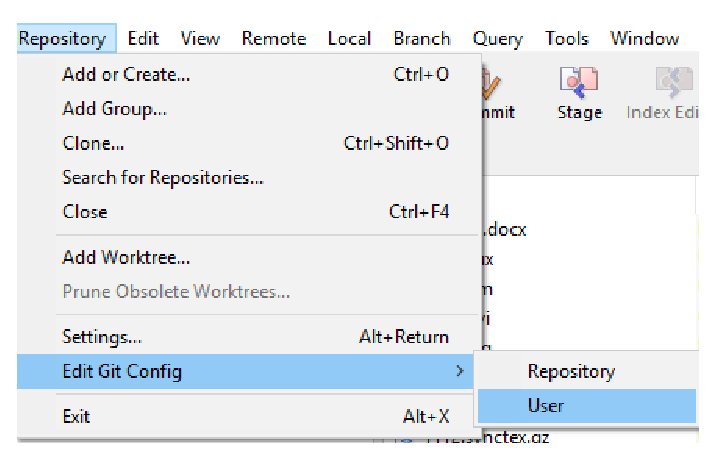
\includegraphics[width=0.75\linewidth]{figures//writing-tools//user_config1.eps}
		\end{figure}
	}{
		\begin{figure}
			\centering
			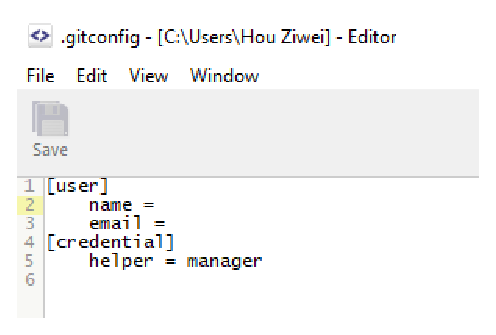
\includegraphics[width=0.75\linewidth]{figures//writing-tools//user_config.eps}
		\end{figure}
	}
	
\end{slide}


\begin{slide}{GitFlow}	
	\begin{figure}
		\centering
		\includegraphics[width=0.45\linewidth]{figures//writing-tools//gitflow.eps}
	\end{figure}
\end{slide}

\begin{slide}[toc=,bm=]{GitFlow}
	\twocolumn{
		\begin{figure}
			\centering
			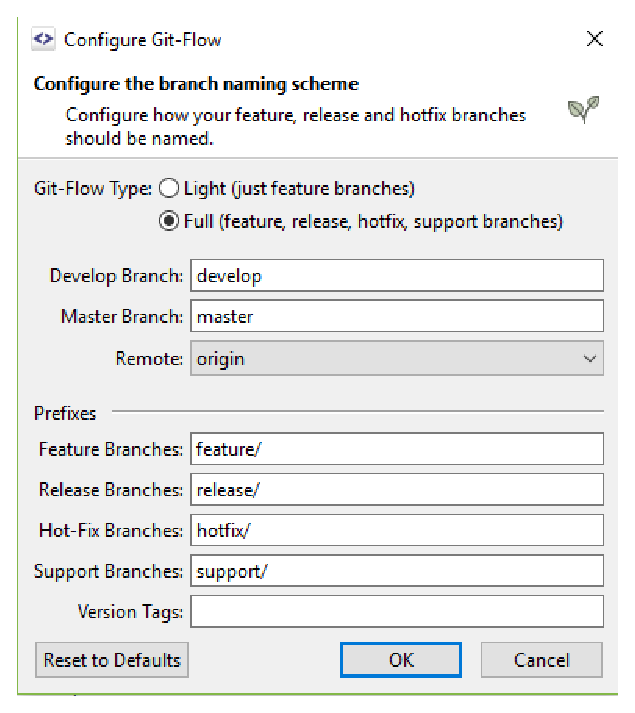
\includegraphics[width=0.75\linewidth]{figures//writing-tools//gitflow2.eps}
		\end{figure}
	}{
		\begin{figure}
			\centering
			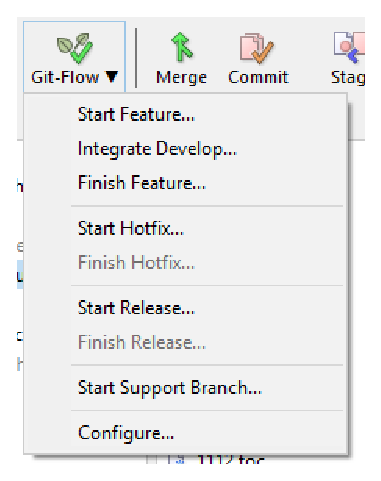
\includegraphics[width=0.75\linewidth]{figures//writing-tools//gitflow3.eps}
		\end{figure}
	}	
	
\end{slide}


\begin{slide}{Rules}
	\begin{itemize}
		\item Put only those files under version control that are directly modified by the user.
		\item Verify that your code can be compiled
		flawlessly before committing your modifications to the repository.
		\item Use compare tools to critically review your modifications before committing them to the repository.
		\item Add a meaningful and descriptive comment when committing your modifications to the repository.
		\item Do not add big files into the repository unless it is really necessary.
	\end{itemize}
\end{slide}


\section{\LaTeX~ \& TeXstudio}

\begin{slide}{Introduce \LaTeX}
	\LaTeX is a high-quality typesetting system; 
	it includes features designed for the production of technical and 
	scientific documentation. 
	\LaTeX is the de facto standard for the communication and publication of 
	scientific documents. \\ 
	To start up \LaTeX editing, 
	MikTex and TeXstudio might be the relative typesetting system and editor need to be installed.\\
%	
%\end{slide}
%
%\begin{slide}{Templates}
	\href{https://github.com/tulip-lab/templatex/tree/develop}{TULIP}
	 provides templates for slides, 
	 paper and thesis.\\
	To use these templates, 
	there are some rules you need to follow. \\
	\begin{itemize}
		\item Avoid ineffective modifications. 
		Do NOT change line breaks without good reasons.
		\item Turn off automatic line wrapping of your Latex editor.
		\item Start each new sentence in a new line.
		\item Split long sentences into several lines so that each line has at 
		most 80 characters.
	\end{itemize}
\end{slide}

\begin{slide}{TeXstudio}
	TeXstudio is a cross-platform open-source LaTeX editor. 
	Its features include an interactive spelling checker, 
	code folding, 
	and syntax highlighting. 
	It does not provide LaTeX itself – 
	the user must choose a distribution of LaTeX and install it first.\\~\\
	
	To start the slides template, 
	there is one configuration you need to set up.
	
	\begin{figure}
		\centering
		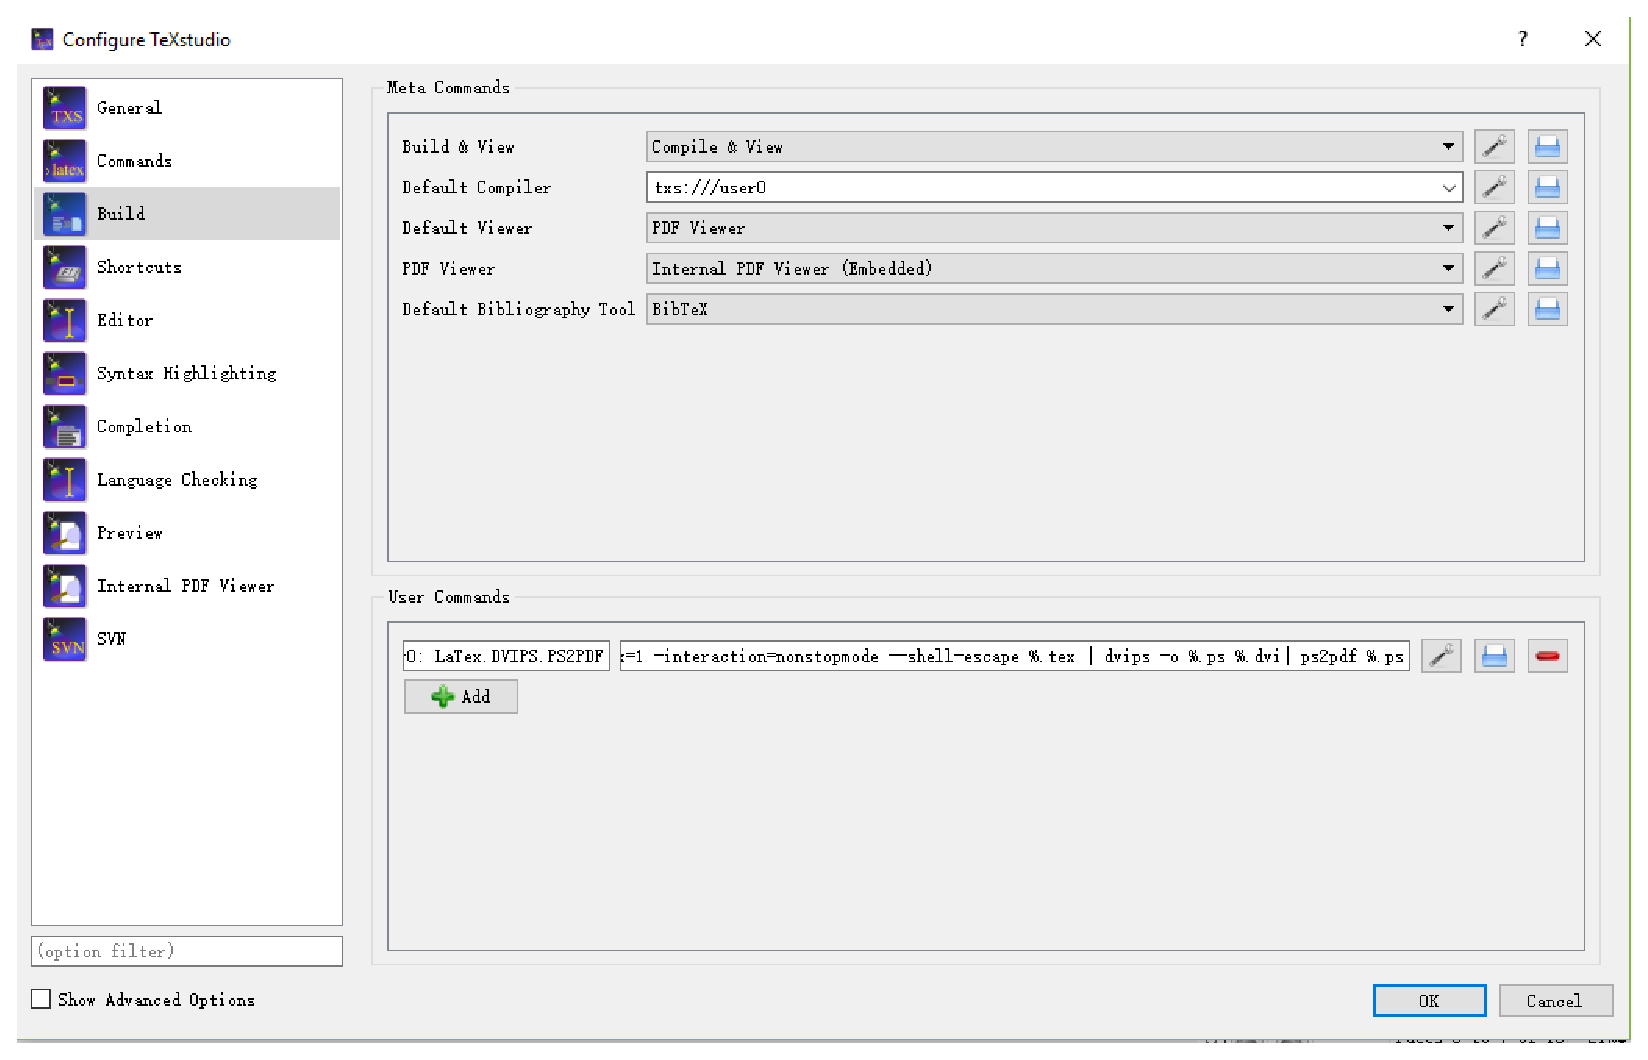
\includegraphics[width=0.75\linewidth]{figures//writing-tools//texstudio_config1.eps}
	\end{figure}

\end{slide}

\begin{slide}{Hints}
	\begin{figure}
		\centering
		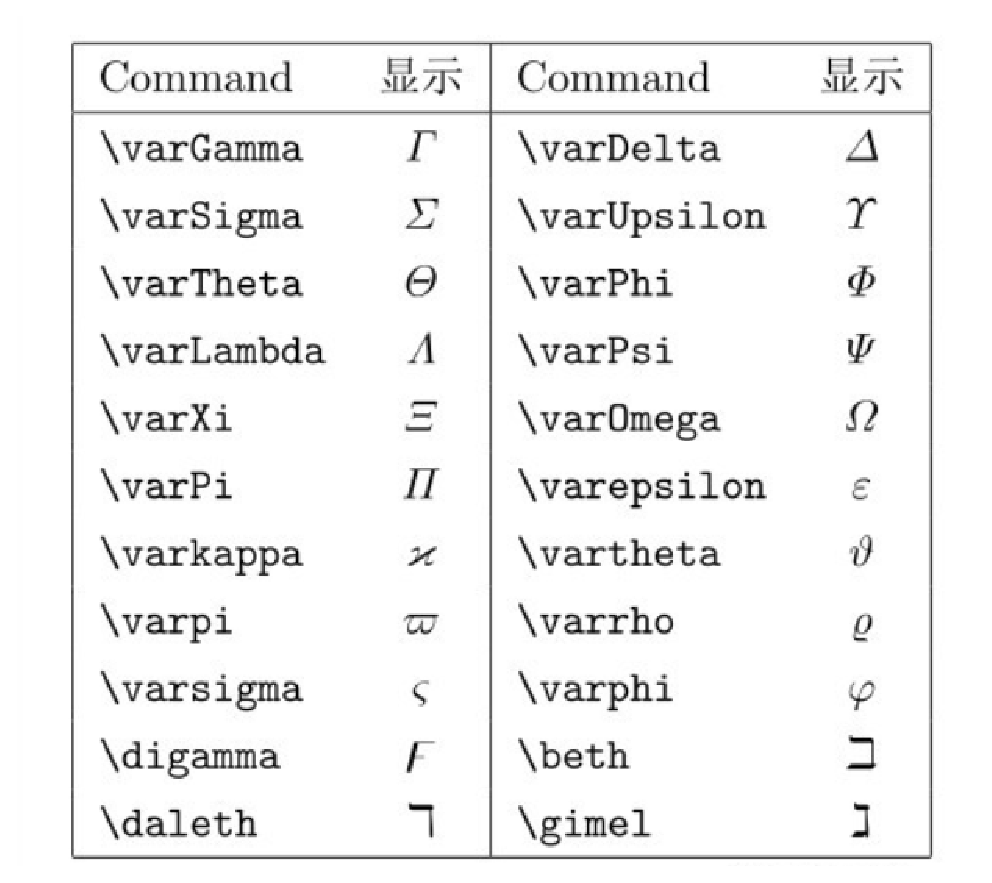
\includegraphics[width=0.45\linewidth]{figures//writing-tools//problems.eps}
	\end{figure}
\end{slide}

\section{Zotero}

\begin{slide}{Zotero}
	Zotero is a free and open-source reference management software to manage 
	bibliographic data and related research materials.\\
	\begin{figure}
		\centering
		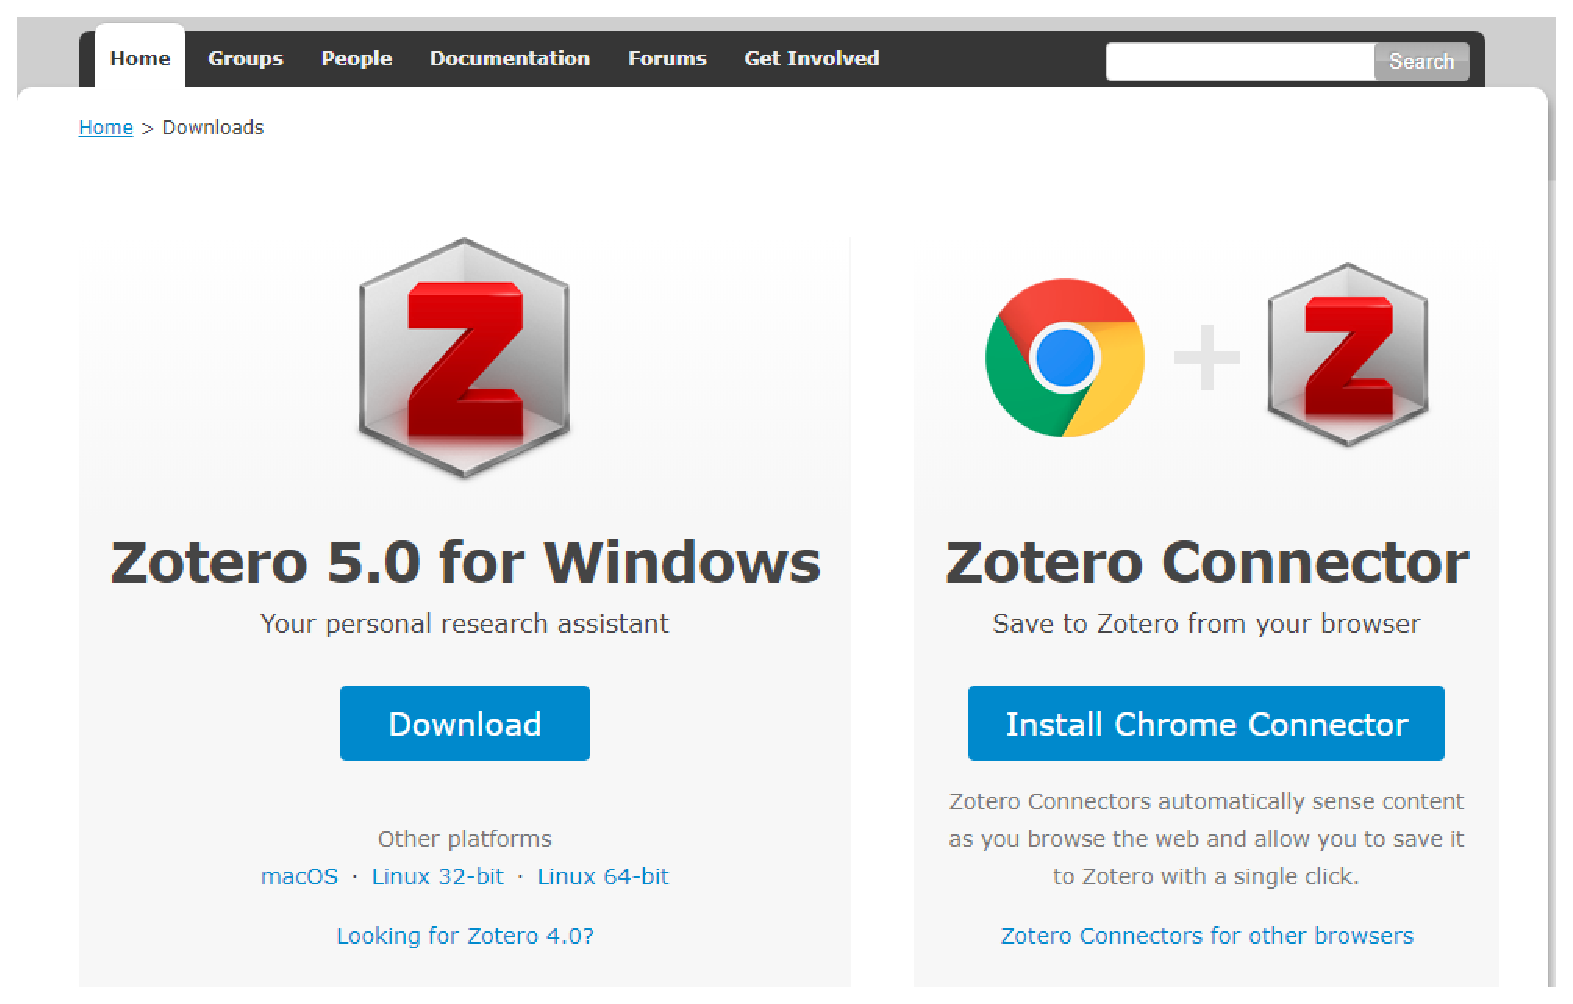
\includegraphics[width=0.6\linewidth]{figures//writing-tools//zotero.eps}
	\end{figure}

\end{slide}



% \begin{slide}{References (1)}
% \bibliographystyle{plain}
% \nobibliography{YourBib}
% \bibentry{someone1}
% \bibentry{someone2}
% \end{slide}
% \begin{slide}{References (2)}
% \bibentry{someone3}
% \end{slide}

% \begin{slide}{Slide}
% \cite{someone}
% \end{slide}
% 
% \begin{slide}{References}
% \bibliographystyle{plain}
% % \bibliography{YourBib}
% \end{slide}


\end{document}

\endinput
